%25.9.2003

\chapter{Gegenbeispiele}
\label{sec:grenzen}

Die in der Einleitung vorgestellte Beziehung zwischen der Perkolationsschwelle und der Nullstelle der mittleren Euler-Charakteristik hat sich in Kapitel \ref{sec:schranken} im Wesentlichen best\"atigt. Auch die Vermutung, dass die Perkolationsschwelle in zwei Dimensionen immer zwischen Wendepunkt und Nullstelle der Euler-Charakteristik liegt, scheint bei einer gro"sen Klasse von Gittern zu stimmen. Es gibt aber auch Gitter, bei denen diese Beziehungen nicht gelten. Im Folgenden sollen diese Gitter vorgestellt und ihre gemeinsamen Eigenschaften identifiziert werden.

\section{site-Perkolation}
Steven van der Marck hat das Quadrat- und das Kagom\'e-Gitter auf verschiedene Arten modifiziert und f\"ur die so erhaltenen zehn neuen Gitter die Perkolationsschwellen numerisch bestimmt. Die Gitter, die van der Marck betrachtet, sind in Abbildung \ref{fig:vandermarck} dargestellt.
\begin{figure}[htbp]
  \centering
  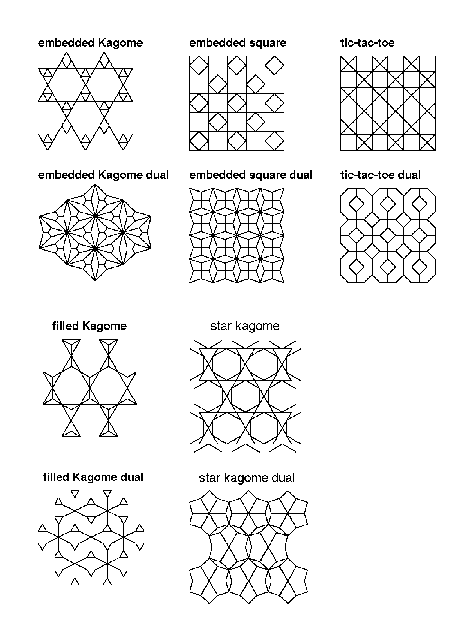
\includegraphics{./Grenzen-Figs/vandermarck}
  \caption{Modifizierte Quadrat- und Kagom\'e-Gitter aus \cite{Marck:03}. }
  \label{fig:vandermarck}
\end{figure}
Die Gitter haben entweder nur zwei Vertextypen, oder bestehen nur aus viereckigen Plaketten. Die Euler-Charakteristiken der Gitter, die nur zwei Vertextypen haben, k\"onnen mit Gleichung (\ref{eq:2-uniform}) ausgerechnet werden. Die Euler-Charakteristiken der \"ubrigen Gitter sind gleich der des Quadratgitters. Die Bezeichungen der Gitter sind in Abbildung \ref{fig:vandermarck} und ihre Vertexkonfigurationen in Tabelle \ref{tab:marckirreg} zu finden. In der Tabelle sind auch die Nullstellen und Wendepunkte der Euler-Charakteristiken und die Perkolationsschwellen der Gitter angegeben.
\begin{table}
\centering
\begin{tabular}{|l|l|r|r||r|}
\hline
Gittername & Vertexkonfiguration & $p_0$ & $p_0^{(2)}$& $p_c$   \\ \hline
\hline

embedded Kagom\'e & $\frac{2}{3}\left[3,3,3,12\right]+\frac{1}{3}\left[3,12,3,12\right]$&0.7580 & $0.6863$&$0.7406(3)$\\ \hline

embedded square & $\frac{2}{3}\left[3,4,3,8\right]+\frac{1}{3}\left[3,8,3,8\right]$&$0.6965$ & $0.6384$&$0.6766(3)$\\ \hline

tic-tac-toe&$ \frac{1}{3}\left[3,3,3,3\right]+\frac{2}{3}\left[3,3,4,3,3,4\right]$&$0.5414$ & $0.5275$&$0.5448(3)$\\ \hline

filled Kagom\'e & $\frac{2}{5}\left[3,3,3\right]+\frac{3}{5}\left[3,3,6,3,3,6\right]$  & $0.6093$ & $0.5754$&$0.6527\dots $ \\ \hline

star Kagom\'e&$ \frac{2}{3}\left[3,6,3,6\right]+\frac{1}{3}\left[3,6,3,6\right]$&$0.6756$ & $0.6231$&$0.7406(2)$ \\ \hline

embedded Kagom\'e dual & wie Quadratgitter &$0.6180$ & $0.5774$&$0.5510(3)$ \\ \hline

embedded square dual &wie Quadratgitter &$0.6180$ & $0.5774$&$0.5770(3)$ \\ \hline

tic-tac-toe dual & $\frac{1}{5}\left[6,6,6,6\right]+\frac{4}{5}\left[4,6,6\right]$&$0.7200$ & $0.6527$&$0.6779(3)$ \\ \hline

filled Kagom\'e dual &$\frac{1}{7}\left[6,6,6,6,6,6\right]+\frac{6}{7}\left[3,6,6\right]$&$0.7156$ & $0.6512$&$0.6599(2)$  \\ \hline

star Kagom\'e dual & wie Quadratgitter&$0.6180$& $0.5774$&$0.5515(2)$  \\ \hline

\end{tabular}
\caption{Die Perkolationsschwelle $p_c$ modifizierter archimedischer Gitter liegt h\"aufig nicht zwischen der Nullstelle $p_0$ und dem Wendepunkt $p_0^{(2)}$ der Euler-Charakteristik. Die Namen der Gitter und die Perkolationsschwellen sind aus \cite{Marck:03} \"ubernommen. ``wie Quadratgitter'' soll bedeuten, dass die Euler-Charakteristik gleich der des Quadratgitters ist. Diese Gitter haben mehr als zwei unterschiedliche Vertextypen, aber nur viereckige Plaketten.}
\label{tab:marckirreg}
\end{table}
Bei vielen dieser Gitter liegt $p_c$ nicht zwischen $p_0$ und $p_0^{(2)}$. Die gr\"o"sten Abweichungen von $p_c$ nach oben sind beim \textit{filled Kagom\'e}- und \textit{star Kagom\'e}-Gitter zu finden. Beim \textit{filled Kagom\'e}-Gitter tragen die Vertices in den Dreiecken des Kagom\'e-Gitters nicht zur Konnektivit\"at bei, denn zwei Vertices auf den Ecken eines Dreiecks sind miteinander verbunden, unabh\"angig davon, ob der Vertex im Dreieck besetzt oder leer ist. Das Gitter perkoliert genau dann, wenn das Kagom\'e-Untergitter perkoliert; $p_c$ ist daher gleich $p_c^{Kagome}=1-2\sin(\pi/18)$. Die Euler-Charakteristiken der beiden Gitter sind aber verschieden. Insbesondere ist die Nullstelle erheblich kleiner, da unbesetzte Vertices in den Dreiecken zus\"atzliche L\"ocher erzeugen k\"onnen.\\
Beim \textit{embedded Kagom\'e dual-} und beim \textit{star Kagom\'e dual}-Gitter ist $p_c$ kleiner als $p_0^{(2)}$. Alle Plaketten dieser Gitter sind Vierecke, und die Euler-Charakteristik ist daher die gleiche wie beim Quadratgitter. Es gibt aber einige Vertices mit hoher und andere mit kleiner Koordinationszahl. Diese Inhomogenit\"at f\"uhrt offensichtlich zu einer Absenkung von $p_c$. Dieser Effekt ist beim \textit{embedded square dual}-Gitter nicht so stark ausgepr\"agt. $p_c$ ist auch dort niedriger als beim Quadratgitter, aber nicht so niedrig wie bei den obigen Gittern und in etwa gleich $p_0^{(2)}$. 

\subsection*{Cluster der Gr\"o"se 1 auf dem \textit{filled Kagom\'e}-Gitter}
Um die Absenkung der Nullstelle der Euler-Charakteristik relativ zur Perkolationsschwelle des \textit{filled Kagom\'e}-Gitters zu untersuchen, bestimmen wir die Beitr\"age der Cluster und L\"ocher der Gr\"o"se 1 zur Euler-Charakteristik. Ein Cluster der Gr\"o"se 1 entsteht, wenn ein Vertex besetzt und alle seine Nachbarn unbesetzt sind. 
\\Die Vertices innerhalb der Dreiecke haben drei Nachbarn und stellen $\frac{2}{5}$ der Vertices. Die \"ubrigen Vertices haben sechs Nachbarn. Die erwartete Zahl der Cluster der Gr\"o"se 1 ist also
\begin{equation}
  n_1(p)=\frac{2pq^3+3pq^6}{5},
\end{equation}
wobei $q=1-p$ ist. Auf dem matching-Gitter haben die Vertices in den Dreiecken die gleiche Nachbarzahl, w\"ahrend die \"ubrigen Vertices zw\"olf Nachbarn haben. F\"ur erwartete Zahl der Cluster der Gr\"o"se 1 auf dem matching-Gitter erh\"alt man also
\begin{equation}
  n_1^*(p)=\frac{2pq^3+3pq^{12}}{5}.
\end{equation}
Im Abschnitt \ref{sec:scaling} wurde die Euler-Charakteristik $\chi_{s_0}(p)$, eingeschr\"ankt auf Cluster und L\"ocher der Gr\"o"se $s\geq s_0$, betrachtet. Zieht man $n_1(p)-n_1^*(q)$ von der Euler-Charakteristik $\chi^{f-Kagome}(p)$ des \textit{filled Kagom\'e}-Gitters ab, erh\"alt man $\chi^{f-Kagome}_2(p)$. Die Nullstelle und der Wendepunkt von $\chi^{f-Kagome}_2(p)$ liegen bei $p_0=0.6804$ und $p_0^{(2)}=0.6220$. Das blo"se Abziehen der Beitr\"age kleinster Cluster ``repariert'' also die Abweichung von $p_0>p_c>p_0^{(2)}$.

\section{bond-Perkolation}
Die Perkolationsschwelle des archimedischen Gitters mit Vertexkonfiguration $(3,4,3,6)$ liegt oberhalb der Nullstelle der Euler-Charakteristik, obwohl $p_c>\frac{1}{2}$ ist. Die Abweichung ist aber nur gering und $p_c$ nur numerisch bekannt.\\
Ein Gegenbeispiel mit exakt bekannter Perkolationsschwelle erh\"alt man, indem jede Gitterkante des Sechseckgitters durch den Graphen, der in Abb. \ref{fig:hexbond} angegeben ist, ersetzt wird.
\begin{figure}[htbp]
  \centering
  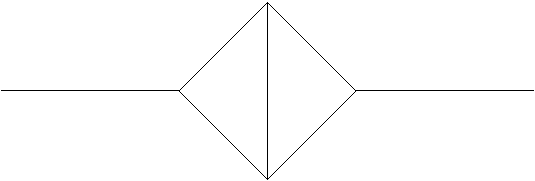
\includegraphics{./Grenzen-Figs/figure}
  \caption{Graph, durch den die Gitterkanten des Sechseckgitters ersetzt werden.}
  \label{fig:hexbond}
\end{figure}
Die bond-Perkolationsschwelle des Sechseckgitters ist exakt bekannt. Die Perkolationsschwelle des modifizierten Gitters ergibt sich aus der Bedingung, dass die Wahrscheinlichkeit, dass der Graph aus Abb. \ref{fig:hexbond}, durchg\"angig ist, gleich der bond-Perkolationsschwelle des Sechseckgitters ist.\\
Diese Wahrscheinlichkeit kann durch Abz\"ahlen aller Konfigurationen ausgerechnet werden. Die beiden Kanten an den Enden des Graphens m\"ussen offen sein, daher ein Faktor $p^2$. Der Graph ist sicherlich durchg\"angig, wenn h\"ochstens eine der mittleren Kanten geschlossen ist, daher ein Beitrag $p^5+5p^4q$. Es gibt zwei M\"oglichkeiten, von den f\"unf mittleren Kanten zwei zu schlie"sen, so dass keine Verbindung von links nach rechts existiert. Es bleiben acht offene Konfigurationen mit zwei geschlossenen Kanten, und man erh\"alt einen Beitrag $8p^3q^2$. Sind nur zwei der f\"unf Kanten offen, gibt es zwei M\"oglichkeiten f\"ur eine offene Verbindung und daher einen Beitrag $2p^2q^3$. Ist nur eine der f\"unf Kanten offen, ist die Verbindung unterbrochen. $p_c$ ist also L\"osung der Gleichung
\begin{equation}
  1-2\sin\left(\frac{\pi}{18}\right) =p^2(p^5+5p^4q+8p^3q^2+2p^2q^3).
\end{equation}
Die einzige L\"osung zwischen null und eins ist $p_c=0.833702\ldots$.\\
Die Euler-Charakteristik des \"Uberdeckungsgitters l\"asst sich mit Gleichung (\ref{eq:matchingpoly}) ausrechnen, und man erh\"alt
\begin{equation}
  \chi(p)=-q+2(1-p^2)-\frac{20}{21}(1-p^3)-\frac{1}{21}(1-p^{24}).
\end{equation}
$\chi(p)$ hat eine Nullstelle bei $p_0=0.82208$; $p_0$ ist also kleiner als $p_c$. Durch das explizite Einf\"uhren einer Substruktur wird auch hier die Euler-Charakteristik abgesenkt, und die Nullstelle ``rutscht'' unter $p_c$.

\section{Eine Folge von Gittern mit $p_c=\frac{1}{2}$ und variierender Euler-Charakteristik}
Ausgehend von einem Dreiecksgitter, wird eine Folge von Gittern $\{\mathcal{G}_n\}$ konstruiert, deren mittlere Euler Charakteristik f\"ur $n=0$ die des Dreiecksgitter ist, und f\"ur $n \rightarrow \infty$ gegen die des Quadratgitters konvergiert. F\"ur alle $n$ ist die site-Perkolationsschwelle $p_c=\frac{1}{2}$.\\
Die Gitter entstehen, wenn man in jedes Dreieck des Dreiecksgitter ein weiteres Dreieck setzt, und dessen Ecken mit den Ecken des \"au"seren Dreiecks verbindet. Die Perkolationsschwelle des Gitters \"andert sich dadurch nicht, da die Vertices an den Ecken des \"au"seren Dreiecks ohnehin miteinander verbunden sind. In das innere Dreieck wird eine Pyramide aus Quadraten eingeschrieben (siehe Abb. \ref{fig:seqgitter}).
\begin{figure}[tbp]
  \centering
  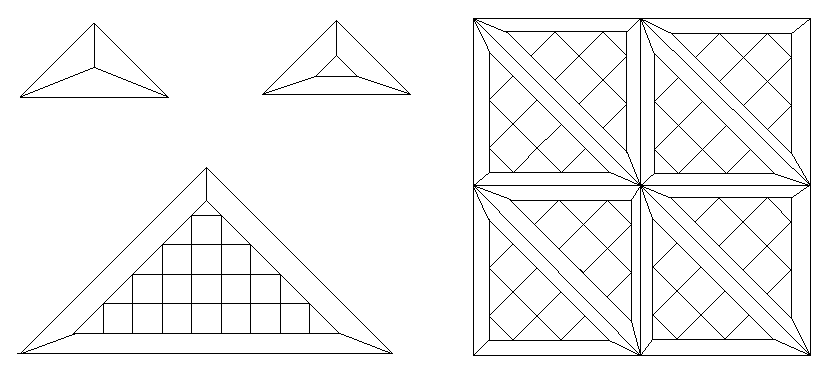
\includegraphics{./Grenzen-Figs/seqgitter}
  \caption{Links: In die Dreiecke eines Dreiecksgitter wird eine Substruktur eingef\"uhrt. Diese Substrukturen sind f\"ur $n=0$, $n=1$ und $n=5$ gezeigt. Rechts ist ein gr\"o"serer Ausschnitt des Gitters mit $n=3$ zu sehen.}
  \label{fig:seqgitter}
\end{figure}
\\Die F\"alle $n=1$ und $n=0$ m\"ussen gesondert betrachtet werden (siehe Abb. \ref{fig:seqgitter}). F\"ur $n=0$ entartet das eingeschriebene Dreieck zu einem Vertex, f\"ur $n=1$ ist das innere Dreieck leer.\\
Die Euler-Charakteristik l\"asst sich mit den bekannten Methoden ausrechnen, und man erh\"alt eine Folge von Nullstellen $p_{n_0}$. Die Folge der Nullstellen hat bei $n=6$ ein Maximum und konvergiert dann langsam gegen $p_0=0.618$ des Quadratgitters (siehe Abb. \ref{fig:sequenze}). 
\begin{figure}[tbp]
  \centering
  \includegraphics{./Grenzen-Figs/sequenze1}
  \caption{Die Nullstellen $p_{n_0}$ der mittleren Euler-Charakteristik der Gitter $\mathcal{G}_n$. Die beiden horizontalen Linien markieren die Perkolationsschwelle der Gitter $p_c=\frac{1}{2}$ und die Nullstelle der Euler-Charakteristik des Quadratgitters $p_0^{sq}=0.618$.}
  \label{fig:sequenze}
\end{figure}\\

Der Zusammenhang zwischen den Nullstellen der Euler-Charakteristik und Perkolationschwellen kann offensichtlich durch Substrukturen zerst\"ort werden. Die Perkolationsschwelle und die Nullstelle der Euler-Charakteristik reagieren unterschiedlich auf Substruktur. W\"ahrend die mittlere Euler-Charakteristik nur durch lokale Beitr\"age erzeugt wird, h\"angen Perkolationsschwellen vor allem von globalen Eigenschaften des Gitters ab. Substrukturen sind f\"ur Perkolation irrelevant und k\"onnen renormiert werden. Im Abschnitt \ref{sec:scaling} wurde schon erw\"ahnt, dass $p_c<p_0$ dann gelten sollte, wenn sich das Skalenverhalten gro"ser Cluster qualitiv auf kleine Cluster fortsetzt. Bei Gittern mit Substruktur ist aber gerade das nicht der Fall.


\section[Gegenbeispiele -- Kontinuumsperkolation]{Kontinuumsperkolation von Kreisringen oder Kugeln verschiedener Radii}
Auch bei Kontinuumsperkolation kann man F\"alle finden, in denen aus der mittleren Euler-Charakteristik keine sinnvollen Aussagen \"uber Perkolationsschwellen gewonnen werden k\"onnen. Das einfachste Beispiel ist die Perkolation von Kreisringen in zwei Dimensionen. Die Euler-Charakteristik einer Vereinigung von Kreisringen ist immer negativ und kann daher keine Information \"uber $p_c$ liefern \cite{Mecke:94}. Ein anderes Beispiel ist Kontinuumsperkolation von Kugeln zwei verschiedener Radii. Hat ein kleiner Anteil der Kugeln einen gro"sen Radius und die \"ubrigen Kugeln einen sehr kleinen Radius, werden die gro"sen Kugeln bei gen\"ugend hoher Punktdichte perkolieren. Durch die vielen isolierten kleinen Kugeln ist die Euler-Charakteristik aber positiv und bei geeigneter Wahl des Gr\"o"senverh\"altnisses der Kugeln kann die Nullstelle der Euler-Charakteristik zu beliebig hohen Punktdichten verschoben werden, obwohl die gro"sen Kugeln perkolieren. Untersuchungen zur Abh\"angigkeit der Perkolationsschwelle und Euler-Charakteristik von Polydispersit\"at sind in Ref. \cite{Mecke:02} zu finden.